%%% Copyright (C) 2018 Vincent Goulet
%%%
%%% Ce fichier fait partie du projet
%%% «Programmer avec R»
%%% https://gitlab.com/vigou3/programmer-avec-r
%%%
%%% Cette création est mise à disposition selon le contrat
%%% Attribution-Partage dans les mêmes conditions 4.0
%%% International de Creative Commons.
%%% https://creativecommons.org/licenses/by-sa/4.0/

\chapter{Éléments d'informatique pour programmeurs}
\label{chap:informatique}

\begin{objectifs}
\item Expliquer la nature de la programmation informatique et le rôle
  des langages.
\item Définir le concept d'algorithme.
\item Comparer la performance d'algorithmes à l'aide de la notation
  $O()$.
\item Identifier les principaux paradigmes de programmation.
\item Distinguer les concepts de syntaxe et de sémantique d'un langage
  de programmation.
\item Distinguer les concepts de langage compilé et de langage
  interprété.
\item Nommer et ordonner les grands jalons de l'histoire des langages
  de programmation.
\item Comprendre la structure du système de fichiers d'un ordinateur
  et identifier le chemin d'accès vers une ressource dans celui-ci.
\end{objectifs}

Vous savez programmer.

En effet, avec l'omniprésence des outils numériques dans notre vie
quotidienne, nous automatisons tous certaines tâches:
%%
demander une alarme pour le lendemain matin;
enregistrer une émission de télé qui sera diffusée dans trois jours;
planifier des virements chez notre institution
  financière;
signaler du contenu ou interpeller quelqu'un sur les médias sociaux
  à l'aide de symboles spéciaux (comme \code{\#} et \code{@});
entrer un code de triche dans un jeu vidéo;
calculer la moyenne d'une colonne dans un tableur;
guider un robot vers la sortie d'un labyrinthe.
%%
Vous pouvez sans doute ajouter vos propres exemples à cette liste.

Dans chacun des exemples précités, vous dictez à une machine des
tâches à effectuer en utilisant un langage qu'elle est à même de
comprendre. Que le langage soit excessivement simple ou qu'une
interface vous guide pas à pas dans la programmation n'y change
fondamentalement rien: vous programmez. Cet ouvrage vise simplement à
vous faire atteindre un niveau de sophistication bien plus grand, un
niveau qui fera réellement de vous des programmeuses et des
programmeurs informatiques.


\section{Qu'est-ce que programmer?}
\label{sec:informatique:programmer}

Programmer est une activité scientifique consistant d'abord et avant
tout à \emph{résoudre des problèmes}. Plutôt que d'avoir recours aux
mathématiques ou à l'expérimentation, les programmeurs demandent à une
machine de résoudre le problème pour eux. Comme le souligne
\citet{Swinnen:python:2012} --- dont la lecture du chapitre~1 est
chaudement recommandée --- programmer est «une compétence de haut
niveau, qui implique des capacités et des connaissances diverses: être
capable de (re)formuler un problème de plusieurs manières différentes,
être capable d’imaginer des solutions innovantes et efficaces, être
capable d’exprimer ces solutions de manière claire et complète.»

La première difficulté réside toutefois dans le fait de «demander» à
une machine de résoudre un problème: il faut établir un mode de
communication pour que l'humain puisse dicter des instructions à une
machine qui, en définitive, ne comprend que deux instructions: vrai et
faux, ouvert ou fermé, 0 ou 1. C'est là le rôle du \emph{langage de
  programmation}.

Tout au long de leur histoire, les humains ont inventé une multitude
de langages pour échanger entre eux: langues parlées, écritures,
langues des signes, peinture, musique, etc. Certains langages
parviennent à mieux exprimer certaines réalités ou certains sentiments
que d'autres. Or, il en va de même des langages de programmation: non
seulement sont-ils nombreux, mais certains conviennent mieux à
certains types de tâches que d'autres. Vous serez à même d'apprécier
la diversité des langages de programmation à la lecture de la
\autoref{sec:informatique:historique} qui retrace les grands jalons de
leur histoire.

\section{Quelques concepts fondamentaux}
\label{sec:informatique:concepts}

Cette section introduit quelques concepts avec lesquels il s'avère
utile d'être familier avant de se lancer dans l'étude de la
programmation. Nous aurons l'occasion de revenir sur ceux-ci plus loin
dans l'ouvrage.

\subsection{Algorithme}
\label{sec:informatique:concepts:algorithme}

Vous avez probablement déjà trié une liste de mots à l'aide d'un
ordinateur. Pourtant, l'ordinateur n'a aucune connaissance du concept
d'ordre alphabétique. Et même s'il «connaissait» cet ordre, comment au
juste réalise-t-il l'opération de tri? Ce genre de questions relève
d'une pierre d'assise de l'informatique:
l'\index{algorithmique}algorithmique, la science qui étudie les
algorithmes et les structures de données.

Un \index{algorithme}\emph{algorithme} est une procédure de calcul
permettant de résoudre un problème bien spécifié. En cela,
l'algorithme explique comment, à partir d'entrants, obtenir l'extrant
solution du problème. Quand on y pense, ce n'est pas très différent
d'une recette culinaire où les entrants sont les ingrédients, la
procédure les étapes de la recette et les extrants, le mets.

L'algorithmique est une discipline riche en techniques ingénieuses et
en analyses mathématiques poussées. Connaitre ses principes de base et
les algorithmes classiques permet de mieux planifier ses méthodes de
résolution de problème. En effet, un bon algorithme permet de résoudre
en quelques secondes un problème qui pourrait autrement prendre des
années.

À titre d'exemple, supposons que vous devez calculer, pour un jeu de
données quelconque, l'écart moyen des données supérieures à $12$ par
rapport à cette valeur. Un premier algorithme de très haut niveau
permettant de résoudre ce problème irait comme suit.

\begin{Schunk}
  \begin{enumerate}
  \item Sélectionner les données supérieures à $12$.
  \item Soustraire $12$ de chaque valeur retenue à la première étape.
  \item Effectuer la moyenne des valeurs obtenues à la seconde étape.
  \end{enumerate}
\end{Schunk}

Apportons une toute petite modification à l'algorithme ci-dessus.

\begin{Schunk}
  \begin{enumerate}
  \item Sélectionner les données supérieures à $12$.
  \item Effectuer la moyenne des valeurs obtenues à la première étape.
  \item Soustraire $12$ de la valeur retenue à la seconde étape.
  \end{enumerate}
\end{Schunk}

Mathématiquement, les deux approches sont tout à fait équivalentes.
Cependant, avec la première approche, nous effectuons une soustraction
pour chaque valeur supérieure à $12$ que compte le jeu de données. Avec
la seconde approche, nous n'effectuons qu'une seule soustraction. Si
le jeu de données compte un million d'entrées supérieures à $12$,
c'est un million de soustractions contre une seule. En temps de
calcul, cela ne représente qu'un écart de quelques centièmes de
secondes sur un ordinateur moderne, mais ces fractions de secondes
peuvent finir par faire une différence importante lorsque la taille
des jeux de données augmente ou lorsque l'opération se répète de
nombreuses fois.

Attardons-nous à un second exemple intéressant: l'élévation d'une
valeur $b$ à la puissance $n$. Un premier algorithme, écrit cette fois
en \index{pseudo-langage}\emph{pseudo-langage}, pourrait se lire
ainsi.

\begin{Schunk}
\begin{Verbatim}
Puissance(nombre réel b, entier n)
  Si n = 0, retourner 1.
  Retourner b * Puissance(b, n - 1).
Fin Puissance
\end{Verbatim}
\end{Schunk}

Cet algorithme est \index{algorithme!récursif}\emph{récursif}: la
procédure \code{Puissance} s'appelle elle-même à répétition jusqu'à
l'obtention du résultat désiré. Mathématiquement, l'algorithme revient
à calculer $b^n$ de la manière la plus simple et intuitive qui soit:
\begin{equation*}
  b^n = b (b (b \cdots (b))).
\end{equation*}
Cela peut convenir lorsque $n$ est petit, mais peut-on faire mieux
pour une «grande» valeur de $n$? Imaginez que vous ne disposez que
d'une calculatrice munie des opérations arithmétiques de base et du
carré, et que vous devez élever un nombre à la puissance, disons,
$21$. Comment feriez-vous pour réduire le nombre d'opérations à entrer
au clavier?

\notebox{Cet exemple est moins fantaisiste qu'il n'y parait! Jusqu'au
  milieu des années 1990, les étudiants en actuariat ne disposaient
  que de ce type de calculatrice pour les examens professionnels. Il
  s'agissait d'un modèle de Texas Instruments affectueusement surnommé
  «TI-0».}

Vous avez pensé à un «algorithme»? Votre idée consiste fort
probablement à diviser la puissance par deux autant de fois que
possible et à élever au carré par la suite. Dans notre exemple, cela
donne
\begin{align*}
  b^{21}
  &= b (b^{20}) \\
  & = b (b^{10})^2 \\
  &= b ((b^5)^2)^2 \\
  & = b ((b (b^4))^2)^2 \\
  &= b ((b (b^2)^2)^2)^2.
\end{align*}
Ce calcul se traduit en algorithme comme suit.

\begin{Schunk}
\begin{Verbatim}
Puissance(nombre réel b, entier n)
  Si n = 0, retourner 1.
    Si n est pair, retourner (Puissance(b, n/2))^2.
    Si n est impair, retourner b * Puissance(b, n - 1).
Fin Puissance
\end{Verbatim}
\end{Schunk}

Pour élever un nombre à la puissance $21$, le premier algorithme
requiert $20$ opérations et le second, seulement $6$. Le dénombrement
du nombre d'opérations requis par un algorithme est un aspect
important de leur analyse. Il se fait généralement en notation $O()$
qui signifie «de l'ordre de». Dans le premier algorithme de calcul de
$b^n$, le nombre d'opérations est directement proportionnel à $n$,
donc on dit que l'algorithme est $O(n)$. Dans le second algorithme où
la puissance est divisée par deux à répétition, le nombre d'opérations
est proportionnel au logarithme (en base deux) de $n$, d'où un
algorithme $O(\log n)$. Pour en savoir plus, consultez
\citet[chapitre~1]{Stephens:algorithms:2013}, qui explique à la fois
très clairement et de manière concise les principes de base du
dénombrement des opérations d'un algorithme.

\citet{Kernighan:practice:1999} font remarquer, fort à propos:
\begin{quote}
  Tous les programmes reposent sur des algorithmes et des structures
  de données, mais très peu de programmes exigent d'en concevoir de
  nouveaux.
\end{quote}
Autrement dit, aussi complexe soit-il, un programme repose souvent sur
quelques algorithmes fondamentaux bien connus et bien établis. À ce
titre, les algorithmes de tri et de recherche jouent un rôle
particulièrement important: on estime que 25~\% du temps de calcul des
ordinateurs dans le monde est consacré au tri et à la recherche! Ce
n'est pour rien que Donald Knuth consacre un volume entier de son
œuvre monumentale \emph{The Art of Computer Programming} à ce seul
sujet \citep{Knuth:ACP:vol1:1997}.

L'étude des algorithmes classiques de tri et de recherche fera l'objet
du \autoref{chap:algorithmique}.


\subsection{Sémantique et syntaxe}
\label{sec:informatique:concepts:semantique}

Il y a plusieurs parallèles à dresser entre les langages de
programmation et les langues parlées ou écrites: leur apprentissage
requiert de la pratique; on en connait jamais un trop grand nombre; le
premier est plus difficile à apprendre que les suivants.
L'informatique a également emprunté à la linguistique les notions de
\index{sémantique}sémantique et de \index{syntaxe}syntaxe.

La sémantique est l'étude de ce que signifie un message ou un
programme informatique, c'est-à-dire de ce qu'il transmet ou exécute.
La syntaxe, quant à elle, étudie la structure du message ou du
programme. En simplifiant, disons que, pour une langue donnée, un
dictionnaire permet de connaitre la sémantique, alors qu'une grammaire
décrit la syntaxe \citep{Hebenstreit:semantique}.

Par exemple, exprimons le message «J'ai soif» en anglais. Dire
«\emph{I am hungry}» relèverait d'une erreur de sémantique, puisque la
signification du message s'en trouve changée. En revanche, avec
«\emph{I have thirsty}», le bon message se rendra, mais peut-être pas
sans que l'erreur de syntaxe n'ait d'abord suscité une hésitation chez
l'interlocuteur\footnote{%
  La formule correcte est «I am thirsty», soit littéralement «Je suis
  soif», en français.}.

Comme pour une langue, la maitrise d'un langage de programmation exige
de respecter à la fois les règles de sémantique et les règles de
syntaxe du langage. Le second volet est relativement facile: si le
programme compile ou s'exécute, c'est généralement que la syntaxe est
respectée. Le respect de la sémantique, ou de la manière propre d'un
langage d'exprimer des idées, demande plus d'efforts et de pratique.


\subsection{Langages compilés et interprétés}
\label{sec:informatique:concepts:compile_vs_interprete}

Tous les langages de programmation\footnote{%
  À l'exception du langage machine, mais rares sont les personnes qui
  ne souhaitent programmer qu'avec des $0$ et des $1$.} %
requièrent un traitement afin que les programmes écrits avec ceux-ci
puissent être exploités par un ordinateur. Il existe deux grandes
façons d'effectuer ce traitement: par compilation et par
interprétation.

Un \index{compilateur}compilateur est un programme informatique qui
transforme en langage machine le code source rédigé dans un langage
donné. On dit alors de ce langage qu'il est \index{compilé
  (langage)}\emph{compilé}. Le compilateur produit un fichier
informatique que l'ordinateur peut ensuite exécuter directement. Sur
la plateforme Windows, on reconnait notamment ces fichiers par leurs
extensions \code{.exe} ou \code{.dll}. Les noyaux d'à peu près toutes
les applications sur nos ordinateurs sont des fichiers compilés.

Un \index{interpréteur}interpréteur, quant à lui, est un programme qui
analyse, traduit et exécute le code source d'un programme
informatique, et ce, à chaque fois que le programme doit être exécuté.
Un langage qui nécessite l'intermédiaire d'un interpréteur est dit
\emph{interprété}. Un programme écrit dans un \index{interprété
  (langage)}langage interprété ne peut être distribué sans son
interpréteur.

Le traitement additionnel entre le code source et le langage machine
fait généralement en sorte que les langages interprétés sont plus
lents que les langages compilés à l'exécution. En revanche, une foule
de détails de mise en œuvre sont pris en charge par l'interpréteur, ce
qui réduit le temps de développement.


\subsection{Paradigmes de programmation}
\label{sec:informatique:concepts:paradigmes}

Un programme informatique est toujours écrit pour résoudre un problème
donné. Or, comme pour tout problème dans la vie, la solution à
celui-ci peut être formulée de différentes manières. Le style
fondamental avec lequel on exprime la solution est appelé le
\index{paradigme}\emph{paradigme} de programmation.

Il existe plusieurs paradigmes de programmation. Nous nous
contenterons ici de se pencher sur seulement quatre.

\begin{description}
\item[Impératif] \index{paradigme!impératif} On indique à l'ordinateur
  les opérations à exécuter et l'ordre dans lequel les exécuter. C'est
  le paradigme le plus intuitif.
\item[Déclaratif] \index{paradigme!déclaratif} On indique cette fois à
  l'ordinateur ce que l'on souhaite obtenir comme résultat, mais sans
  préciser comment y parvenir. Il est laissé à la mise en œuvre du
  langage de déterminer la meilleure méthode de résolution du
  problème.

  Par exemple, pour extraire d'une base de données \code{etudiants} le
  prénom de toutes les personnes de plus de 25~ans, on écrira dans un
  langage déclaratif comme le SQL:
\begin{Schunk}
\begin{Verbatim}
SELECT prenom FROM etudiants WHERE age > 25
\end{Verbatim}
\end{Schunk}
  Nulle part n'est-il précisé comment le programme devrait procéder à
  l'extraction.
\item[Fonctionnel] \index{paradigme!fonctionnel} Un programme est une
  suite d'appels de fonctions, comme en mathématiques. L'exécution
  d'une fonction n'a pas d'impact sur les autres fonctions\footnote{%
    Autrement on dit qu'une fonction a un effet de bord (\emph{side
      effect}).} %
  Les opérations complexes sont réalisées en combinant les fonctions,
  de manière analogue à la composition de fonctions $g \circ f$.
\item[Orienté objet] \index{paradigme!orienté objet} Un programme est
  conçu comme un ensemble de blocs logiciels (les objets) qui
  interagissent entre eux. Une \emph{méthode} applique un traitement
  différent à un objet selon sa \emph{classe}. Ce paradigme est
  particulièrement utilisé dans les grands et complexes projets
  informatiques.
\end{description}

La plupart des langages d'usage courant combinent d'office, ou du
moins permettent de combiner, plusieurs paradigmes. Par exemple, le
langage {\Cpp} est à la fois un langage impératif et orienté objet.


\section{Bref historique des langages de programmation}
\label{sec:informatique:historique}

Ada Lovelace (1815--1852) est généralement reconnue comme la première
autrice d'un algorithme et de ce que l'on appelle aujourd'hui un
programme informatique. C'est en son honneur qu'a été nommé le langage
Ada conçu en réponse à un cahier de charges du département de la
Défense des États-Unis au début des années 1980.

Franchissons d'un bond les premiers jours de l'informatique et de la
programmation pour arriver aux ordinateurs électriques modernes, dans
les années 1940. On programme alors ceux-ci en
\index{assembleur}assembleur, un langage de très bas niveau conçu pour
faciliter l'entrée de programmes dans un ordinateur
(\autoref{fig:informatique:assembleur}). Le langage demeure loin
d'être facile à déchiffrer, mais c'est toujours préférable au langage
machine, constitué uniquement de 0 et de 1. Le coût d'utilisation d'un
ordinateur est à l'époque bien supérieur à celui d'une personne, aussi
la traduction du langage assembleur vers le langage machine
demeure-t-elle confiée à des humains. Au fil des années, le rapport de
coût s'inversera et il deviendra financièrement plus avantageux de
confier cette tâche cléricale à l'ordinateur lui-même, via un
programme d'assembleur\footnote{%
  J'ai tiré cette manière de présenter les choses de
  \cite{Oualline:C:1997}.}.

\begin{figure}
  \centering
  \includegraphics[trim=0 475 0 0, clip=true]{images/Motorola_6800_Assembly_Language.png}
  \caption[Programme en assembleur pour un microprocesseur 8~bits
    Motorola 6800]{Extrait d'un programme en assembleur pour un
    microprocesseur 8~bits Motorola 6800. {\small Source:
      \link{https://commons.wikimedia.org/wiki/File\%3AMotorola_6800_Assembly_Language.png}{Wikimedia
        Commons}}}
  \label{fig:informatique:assembleur}
\end{figure}

Les premiers langages créés pour transmettre des instructions à un
ordinateur tout en demeurant faciles à lire par les humains
apparaissent dans les années 1950. Ils sont à l'origine intimement
liés à l'architecture d'un ordinateur: à chaque type d'ordinateur son
langage de programmation. Certaines contraintes --- ou exigences ---
des langages de l'époque proviennent aussi du support physique alors
utilisé pour stocker les programmes: les cartes perforées.

\subsection{Fortran}
\label{sec:informatique:historique:fortran}

En 1954, l'ingénieur de IBM John Backus publie les spécifications du
langage \index{Fortran}FORTRAN (\emph{FORmula TRANslating System}). Le
premier compilateur voit le jour deux ans plus tard. Fortran (avec des
minuscules à partir de 1977) deviendra rapidement le langage standard
dans le calcul scientifique.

Plus d'un demi-siècle plus tard, l'empreinte de Fortran demeure
importante, notamment grâce aux bibliothèques d'algèbre linéaire
BLAS\footnote{%
  \emph{Basic Linear Algebra Subprograms};
  \link{http://www.netlib.org/blas}{}.} %
et LAPACK\footnote{%
  \emph{Linear Algebra PACKage};
  \link{http://www.netlib.org/lapack}{}.} %
auxquelles ont recours la plupart des progiciels scientifiques, dont
R. Le langage est toujours utilisé en calcul haute performance et pour
mesurer le rendement des superordinateurs.

\notebox{Dans le très recommandable film «Les figures de l'ombre»
  (\emph{Hidden Figures}, 2016), une des héroïnes entreprend de
  s'attaquer à la programmation des nouveaux ordinateurs de la NASA.
  On peut alors voir qu'elle apprend le Fortran.}

\subsection{Lisp}
\label{sec:informatique:historique:lisp}

Le deuxième langage le plus ancien toujours largement diffusé est
\index{Lisp}Lisp (\emph{LISt Processing}). Créé par John McCarthy en
1958 en tant que modèle pratique pour représenter des programmes, le
Lisp est devenu le langage de choix pour la recherche et les
applications en intelligence artificielle. Le terme Lisp désigne
aujourd'hui une famille de langages comprenant de nombreux dialectes,
dont Common Lisp, Scheme et Emacs Lisp.

Le Lisp se distingue en outre par une syntaxe simple en
\index{notation!préfixée}notation préfixée (voir l'encadré à la
\autopageref{fig:informatique:notations}), le support pour la
programmation fonctionnelle
(\autoref{sec:informatique:concepts:paradigmes}) et la faculté de
manipuler le code source en tant que structure de données. Autre trait
distinctif: la syntaxe du Lisp fait un usage immodéré des parenthèses.

\begin{figure}[t]
  \label{fig:informatique:notations}
  \setlength{\FrameRule}{1pt}
  \lstset{backgroundcolor=\color{codebg},
    frame=lr, rulecolor=\color{codebg},
    numbers=none,
    xleftmargin=3.4pt, xrightmargin=3.4pt}
  \begin{emphbox}{\mdseries Notations infixée, préfixée et suffixée}
    Les notations \index{notation!infixée}infixée (\emph{infix}),
    \index{notation!préfixée}préfixée (\emph{prefix}) et
    \index{notation!suffixée}suffixée (\emph{postfix}) sont trois
    manières différentes, mais équivalentes, d'écrire des expressions
    en mathématiques ou en programmation.

    Par exemple, l'opération d'addition de deux opérandes $x$ et $y$
    s'écrit en notation infixée
\begin{lstlisting}
x + y
\end{lstlisting}
    En notation préfixée, aussi appelée notation polonaise,
    l'opérateur est placé avant les opérandes:
\begin{lstlisting}
+ x y
\end{lstlisting}
    On l'aura compris, en notation suffixée, ou notation polonaise
    inversée, l'opérateur apparait après les opérandes:
\begin{lstlisting}
x y +
\end{lstlisting}
    Nous sommes davantage habitués à lire la notation infixée, quoique
    la notation préfixée nous soit familière pour les opérateurs à un
    seul opérande (comme la négation) ou pour les appels de fonctions.
    La notation suffixée n'a jamais recours aux parenthèses.

    La compagnie HP commercialise de très prisées calculatrices
    scientifiques utilisant la notation suffixée (libellées RPN pour
    \emph{Reverse Polish Notation}) depuis 1972.
  \end{emphbox}
\end{figure}

Le Lisp est entouré d'une aura de beauté et d'élégance dont peu
d'autres langages peuvent se targuer. Citons Eric Raymond dans
\link{http://www.catb.org/esr/faqs/hacker-howto.html}{\emph{How to
    Become a Hacker}}:
\begin{quote}
  Il faut apprendre le Lisp pour l'extraordinaire expérience d'éveil
  [\emph{enlightenment experience}] que procure le fait de finalement
  le comprendre; cette expérience fera de vous un meilleur programmeur
  pour toujours, même si vous n'avez plus vraiment à utiliser le Lisp.
\end{quote}

Pour illustrer encore davantage la place toute particulière qu'occupe
le Lisp en programmation, mentionnons également l'aphorisme selon
lequel «ceux qui ne connaissent pas le Lisp sont condamnés à le
réinventer», d'une certaine façon la version courte de la célèbre
\link{https://en.wikipedia.org/wiki/Greenspun\%27s_tenth_rule}{\emph{Greenspun's
    tenth rule of programming}}: %
\begin{quote}
  Tout programme suffisamment complexe en C ou en Fortran comporte une
  mise en œuvre mal spécifiée, pleine de bogues et lente de la moitié
  de Common Lisp.
\end{quote}
(Fait amusant à noter: il n'y a pas d'autres lois que la dixième, de
l'\link{http://philip.greenspun.com/bboard/q-and-a-fetch-msg?msg_id=000tgU}{aveu
  même de l'auteur}.)

\subsection{COBOL}
\label{sec:informatique:historique:cobol}

Le troisième langage développé dans les années 1950 et toujours en
usage de nos jours est \index{COBOL}COBOL (\emph{COmmon Business
  Oriented Language}). Ce langage spécialisé dans les applications de
gestion a été créé en 1959 par un comité formé pour proposer un
langage commun pour l'administration américaine.

Le COBOL reste très utilisé dans de grandes entreprises, notamment
dans les institutions financières. La légende urbaine veut d'ailleurs
que les programmeurs COBOL soient comparativement très bien rémunérés
aujourd'hui sous l'effet combiné de leur rareté et de l'importance
opérationnelle des applications qu'ils doivent maintenir.

\subsection{Algol}
\label{sec:informatique:historique:algol}

Dès la fin de la décennie 1950, un comité de scientifiques se réunit à
Zurich pour concevoir ce que l'on voudrait voir devenir le langage de
programmation standard. De ces rencontres naitra \index{Algol}Algol
(\emph{ALGorithmic Oriented Language}) en 1958. Comme la plupart des
tentatives de définition d'un standard, c'est un échec: le langage est
populaire dans les milieux académiques, mais restera peu utilisé dans
les applications commerciales.

Cela dit, on doit à Algol plusieurs innovations importantes, de telle
sorte qu'un grand nombre des langages qui verront le jour par la suite
seront considérés comme ses descendants; le poster
\link{http://www.oreilly.com/go/languageposter}{\emph{History of
    Programming Languages}} de O'Reilly Media illustre ceci à
merveille. \citet{Hoare:1973} a d'ailleurs cette jolie formule:
\begin{quote}
  Voici un langage très en avance sur son temps, il n'a pas seulement
  été une amélioration de ses prédécesseurs mais aussi une
  amélioration de presque tous ses successeurs.
\end{quote}

\begin{figure}[t]
  \centering
  \begin{minipage}{0.9\linewidth}
    \setkeys{Gin}{width=\textwidth}
    \includegraphics{images/standards} \\
    \footnotesize\sffamily%
    Tiré de \href{http://xkcd.com/927/}{XKCD.com}
  \end{minipage}
\end{figure}

\subsection{APL}
\label{sec:informatique:historique:apl}

Notre historique ne serait pas complet sans un mot sur \index{APL}APL
(\emph{A Programming Language}, qui l'aurait cru). Même s'il n'a
jamais connu une diffusion importante, ce langage conçu par Kenneth
Iverson autour de 1962 n'en a pas moins eu une influence considérable
sur la manière de penser et de représenter les opérations
mathématiques sur les tableaux à plusieurs dimensions.

Doté d'une large gamme de symboles pour représenter des opérations et
d'une syntaxe tout à fait particulière --- les expressions sont
exécutées de droite à gauche! --- l'APL est remarquablement concis et
puissant; voir la \autoref{fig:informatique:apl} pour un aperçu. Le
revers de la médaille et ce qui a assurément nui à son adoption
à large échelle, c'est la difficulté que l'on éprouve à relire le
code. Assez pour que d'aucuns qualifient l'APL de «langage à écriture
seulement».

APL a pendant longtemps été un langage très prisé par les actuaires,
ce qui fait qu'il subsiste des applications dans ce langage dans
certaines compagnies d'assurance. Le modèle de traitement des
vecteurs, matrices et tableaux de l'APL a servi d'inspiration pour la
conception du langage S --- nous y reviendrons au
\autoref{chap:presentation}.

Le langage continue sa vie aujourd'hui principalement sous forme de son
successeur, \index{J}J.

\begin{figure}
  \centering
  \scalebox{0.4}{\includegraphics{images/APL_intro}}
  \caption[Opérations simples en APL]{Opérations simples en APL. De
    haut en bas: génération des nombres de $1$ à $5$ et stockage dans
    la variable \code{x}; affichage du contenu de \code{x}; somme des
    éléments de \code{x}; moyenne des éléments de \code{x}. {\small
      Image: {\textcopyright} François-Dominique,
      \href{https://creativecommons.org/licenses/by-sa/4.0/deed.fr}{CC
        BY-SA 4.0}, via
      \href{https://commons.wikimedia.org/w/index.php?curid=43207460}{Wikimedia
        Commons}}}
  \label{fig:informatique:apl}
\end{figure}

\subsection{C}
\label{sec:informatique:historique:c}

Le langage \index{C}C a été inventé en 1972 chez Bell Labs par Ken
Thompson et Dennis Ritchie afin de réécrire le système d'exploitation
UNIX (\autoref{sec:informatique:os:unix}). Il demeure beaucoup utilisé
pour la programmation système: le noyau de systèmes d'exploitation
comme Windows et Linux sont développés en grande partie en C.

Le C est un langage de programmation généraliste considéré, selon les
standards actuels, comme de bas niveau. Pour illustrer, l'utilisateur
doit programmer des traitements comme la libération de la mémoire, la
vérification de la validité des indices sur les tableaux, l'ouverture
et la fermeture des fichiers, etc.

Le langage demeure l'un des plus utilisés dans le monde et son
influence est considérable. De nombreux langages plus modernes comme
\index{C++@\Cpp}\Cpp, \index{C#@C\#}C\# et \index{Java}Java reprennent des
aspects de C. Le C est également beaucoup utilisé pour le calcul
numérique intensif, où il s'est en quelque sorte substitué à Fortran.
La plupart des progiciels scientifiques --- dont R, encore une fois
--- offrent la possibilité d'appeler du code C lorsque la rapidité de
calcul devient un enjeu. Le gain en temps d'exécution doit toutefois
être suffisamment grand pour compenser le temps de développement plus
long qu'exige le C par rapport à des langages de plus haut niveau.

\notebox{Dans l'ouvrage classique de \cite{KandR:1978}, le premier
  exemple d'un programme C affiche le message «\emph{hello, world}» à
  l'écran. Ça deviendra ensuite une tradition de démontrer le
  fonctionnement ou la syntaxe d'un langage avec cet exemple.}

\subsection{Autres jalons}
\label{sec:informatique:historique:autres}

Nous nous sommes attardés jusqu'ici à des langages de programmation
vieux de plus de 40 ans à cause de leur importance historique et parce
qu'ils sont toujours utilisés couramment. De nombreux autres langages
ont vu le jour depuis, si bien qu'ils se comptent aujourd'hui par
milliers. En voici quelques autres ayant occupé une place
prépondérante dans l'histoire.

\begin{itemize}
\item Comme son nom l'indique, \index{C++@\Cpp}\textbf{\Cpp} (Bjarne
  Stroustrup, 1980) est un dérivé du C qui lui ajoute, en autres
  choses, la programmation orientée objet. Certains considèrent que
  {\Cpp} devrait être le point d'entrée de toute personne voulant
  débuter à programmer avec des langages de la famille du C. Le code C
  est compatible avec le \Cpp.
\item Principal représentant de l'ère Internet des années 1990,
  \index{Java}\textbf{Java} (James Gosling, 1995) a été conçu pour
  que le code écrit dans ce langage puisse s'exécuter sur n'importe
  quelle plateforme informatique sans nécessiter une nouvelle
  compilation. Il est donc très populaire dans les applications web ou
  embarquées. Sa syntaxe est fortement inspirée du \Cpp.
\item \index{Visual Basic}\textbf{Visual Basic} (Microsoft, 1991)
  permet de développer des applications de manière interactive en
  disposant des composantes sur un canevas. Le langage est aujourd'hui
  discontinué, mais son dérivé \textbf{Visual Basic for Applications}
  (\index{VBA}VBA) demeure beaucoup utilisé dans les applications de
  la suite bureautique Office.
\item \index{Python}\textbf{Python} (Guido van Rossum, 1991) est un
  langage de haut niveau, orienté objet, multiplateforme et sous
  licence libre. C'est un des langages les plus utilisés aujourd'hui
  pour le calcul scientifique et l'analyse de données massives.
\end{itemize}

Certains langages de programmation ont une vocation généraliste,
certains visent des niches particulières, alors que d'autres cherchent
surtout à faire progresser l'état des connaissances dans la théorie
des langages. Quoi qu'il en soit, un langage de programmation demeure
un outil et, en informatique comme dans d'autres domaines, il convient
de choisir le meilleur outil pour accomplir une tâche donnée.

J'invite les lecteurs intéressés à en savoir davantage sur
l'histoire des langages de programmation en général, ou sur l'un ou
l'autre des langages mentionnés ci-dessus en particulier, à débuter
par les très complètes entrées de Wikipedia en
\link{https://fr.wikipedia.org/wiki/Histoire_des_langages_de_programmation}{français}
et en
\link{https://en.wikipedia.org/wiki/History_of_programming_languages}{anglais}.
\citet[chapitre~2]{Oualline:C:1997} propose également une excellente
introduction à la notion de programmation ainsi qu'une brève, mais
instructive, histoire du langage C.


\section{Systèmes d'exploitation}
\label{sec:informatique:os}

À titre de (futurs) programmeurs, vous devrez tirer profit au maximum
des ressources de votre ordinateur. Ceci exige d'en connaitre le
fonctionnement mieux que l'utilisateur lambda. Or, vos principaux
outils numériques sont aujourd'hui les téléphones et tablettes aux
interfaces hautement simplifiées. Connaissez-vous le rôle du
système d'exploitation d'un ordinateur? En connaissez-vous les
diverses variantes et leurs caractéristiques principales?
Comprenez-vous bien le système de classification des fichiers de votre
ordinateur? Vous devrez pouvoir répondre «oui» à ces questions. Cette
section et la suivante sont là pour vous y aider.

Le \index{système d'exploitation}système d'exploitation
(\emph{operating system}, OS) est un ensemble de programmes qui gère
les ressources matérielles et logicielles d'un ordinateur. Premier
programme exécuté par l'ordinateur lors de la mise en marche, le
système d'exploitation reçoit les demandes de ressources des
applications --- espace mémoire, unité de calcul, disque dur,
communication avec les périphériques, utilisation du réseau --- et les
alloue en fonction de l'état du système et des demandes concurrentes
des autres applications. Tous les logiciels applicatifs requièrent un
système d'exploitation pour fonctionner.

Il existe une grande variété de systèmes d'exploitation. Les plus
connus aujourd'hui sont, pour les ordinateurs personnels et les
serveurs, Windows de Microsoft, macOS de Apple et Linux, un logiciel
libre créé et toujours administré par Linus Torvalds. Pour les
appareils mobiles, deux systèmes d'exploitation se partagent
l'essentiel du marché: iOS et Android. Le premier est dérivé de macOS
et le second, de Linux.

Les systèmes macOS et Linux appartiennent à la famille des systèmes
Unix. Cela ne laisse donc en fait que deux grandes classes de systèmes
d'exploitation couramment utilisés: Windows et Unix.

\subsection{Windows}
\label{sec:informatique:os:windows}

Le système d'exploitation \index{Windows}Windows de Microsoft équipe
près de 90~\% des ordinateurs personnels dans le monde. Dans les
circonstances, rares sont les personnes qui n'ont jamais utilisé le
système, ne serait-ce qu'à petites doses.

À l'origine, en 1985, Windows n'était qu'une interface graphique
superposée au véritable système d'exploitation des ordinateurs de type
«compatibles IBM PC», le DOS. Les versions grand public depuis
Windows~2000 sont plutôt basées sur le noyau de Windows~NT, un système
conçu à partir de zéro et lancé au milieu des années 1990 en tant que
système pour les entreprises.

Le plus grand avantage de Windows est son ubiquité. À peu près toutes
les applications, sauf peut-être celles s'adressant à un segment de
marché très précis, sont disponibles sous Windows, que ce soit en code
natif, via un port depuis Unix, ou encore par l'intermédiaire d'une
couche logicielle d'émulation comme Cygwin ou \index{MinGW}MinGW.

Un système d'exploitation multiutilisateur prend pour acquis que
plusieurs utilisateurs se partageront les ressources de l'ordinateur,
simultanément lorsqu'il s'agit d'un serveur, ou les uns après les
autres dans le cas d'un ordinateur personnel. Dans un tel système, on
établit des règles strictes d'accès aux ressources du système (seul
l'administrateur peut installer ou supprimer des applications) et
d'accès aux ressources des autres utilisateurs (Marianne n'a pas
accès aux fichiers d'Alexandre et vice-versa).

Les versions de Windows multiutilisateurs sont apparues relativement
tard sur le marché grand public, et ce, sans que le paradigme ne soit
imposé aux utilisateurs. Résultat: la plupart des utilisateurs de
Windows s'octroient à la ronde les droits d'administrateur et, pire,
plusieurs applications nécessitent toujours un accès total au système.
C'est par ces failles que se propagent virus et autres logiciels
malveillants sur la plateforme.

Les systèmes Windows sont livrés avec une trousse de développement
très restreinte. Les programmeurs doivent donc installer les outils
nécessaires, souvent sous forme de suites logicielles monolithiques,
ce qui entraine dédoublements et, parfois, conflits.

\subsection{Unix}
\label{sec:informatique:os:unix}

Le terme \index{Unix}\emph{Unix} --- ou UNIX qui, en majuscules, est
une marque déposée de \link{http://www.opengroup.org/unix}{Open Group}
--- recoupe une famille de systèmes d'exploitation dérivant tous du
premier système Unix développé chez Bell Labs dans les années 1970 par
Kenneth Thompson, Dennis Ritchie et plusieurs autres.

Les systèmes Unix partagent un certain nombre de caractéristiques
communes. D'abord, ils sont intrinsèquement multitâches et
multiutilisateurs. Ensuite, la
\Index{Unix!philosophie}\link{https://fr.wikipedia.org/wiki/Philosophie_d\%27Unix}{philosophie
  Unix} commande la modularité: le système d'exploitation fournit aux
utilisateurs et aux applications une multitude de petits outils très
spécialisés qui ne réalisent à peu près qu'une seule tâche. Le système
rend ensuite simple, via un mécanisme dit de transfert de données
(«tuyau», \emph{pipe}), de les combiner pour effectuer des opérations
plus complexes; nous y reviendrons à la \autoref{sec:cli:flux}.

Par exemple, pour extraire le mot \emph{tuyau} du code source
contenant le précédent paragraphe, nous pourrions utiliser l'outil
\code{grep} pour extraire la ligne où se trouve le mot, puis l'outil
\icode{cut} pour isoler le mot qui nous intéresse et, enfin, l'outil
\icode{tr} pour supprimer la parenthèse ouvrante, les guillemets et la
virgule autour du mot.\footnote{%
  En supposant que le mot recherché est le quatrième de la ligne dans
  le fichier source \code{informatique.tex}, la commande résultante
  est: \code{grep "«tuyau»" informatique.tex | cut -d " " -f 4 | tr -d
    \bs(«»,}\,. Le symbole %
  \index{{"|}@\string\code{\string\textbar} (Bash)}\code{\textbar} %
  est l'opérateur de transfert de données de Unix.%
  %% utilisation de \string: https://tex.stackexchange.com/a/254505
}

À l'exception notable des Mac, \index{Unix}Unix demeure assez peu
répandu sur les ordinateurs personnels. En revanche le système
d'exploitation, en particulier sa variante libre Linux, équipe
l'immense majorité des stations de travail, des serveurs et des
supercalculateurs. De plus, bon nombre d'applications scientifiques et
de langages de programmation sont d'abord développés sur des systèmes
Unix. Pour ces raisons, j'estime utile pour des programmeurs de
connaitre les quelques «Unix-ismes» ci-dessous.

\begin{itemize}
\item La barre oblique (\code{/}) est utilisée pour séparer les
  dossiers dans les chemins d'accès aux fichiers.
\item Tout utilisateur dispose d'un espace disque réservé identifié
  comme le \index{repertoire personnel@répertoire
    personnel}\emph{répertoire personnel} ou le \index{dossier de
    départ|see{répertoire personnel}}\emph{dossier de départ}
  (\emph{home directory}). Ce répertoire est situé dans \code{/Users}
  sous macOS et habituellement dans \code{/home} sous Linux.
\item À la ligne de commande et dans la configuration de plusieurs
  applications, le caractère \,\verb=~=\, représente le répertoire
  personnel.
\item Toujours à la ligne de commande, il est possible d'appuyer sur
  \code{TAB} pour compléter les noms de fichiers, de répertoires ou de
  commandes.
\item Plusieurs applications permettent de stocker des options de
  configuration sous forme de texte brut dans des fichiers dont le nom
  débute généralement par un point «\verb=.=»\,.
\end{itemize}
La section suivante fournit des détails additionnels sur le système de
fichiers de Unix.

\osxbox{Vous savez désormais pourquoi le \index{repertoire
    personnel@répertoire personnel}répertoire personnel, ou \emph{home
    directory}, est représenté par une maison dans le Finder et que le
  raccourci clavier pour y accéder est \code{\shiftkey\,\cmdkey\,H}.}


\section{Systèmes de fichiers}
\label{sec:informatique:fs}

Le \index{système de fichiers}système de fichiers d'un ordinateur
contrôle l'inscription, l'organisation et la récupération des données
sur une unité de stockage, souvent un disque dur.

Nous n'entrerons pas dans les détails techniques des systèmes de
fichiers. Seulement, les programmeurs doivent être familiers avec
quelques grands principes de l'organisation des données dans un
ordinateur.

Les fichiers sont regroupés dans des
\index{repertoire@répertoire}\emph{répertoires} (ou dossiers). Ceux-ci
contiennent eux-mêmes des fichiers ou des sous-répertoires. Ce schéma
se répète sans limite pratique. Il en résulte une classification sous
forme d'arbre dont la \emph{racine} est le répertoire contenant
l'intégralité des fichiers. La \autoref{fig:informatique:fs} présente
des extraits des arbres de fichiers usuels de Windows et de macOS.

\begin{figure}
  \begin{minipage}[t]{0.45\linewidth}
    \dirtree{%
      .1 \code{C:\bs}.
      .2 \code{Program Files\bs}.
      .3 \code{Internet Explorer\bs}.
      .3 \code{Windows NT\bs}.
      .2 \code{Users\bs}.
      .3 \code{Alexandre\bs}.
      .4 \code{Desktop\bs}.
      .4 \code{Documents\bs}.
      .5 \code{synthese-1.doc}.
      .2 \code{Windows\bs}.
      .3 \code{explorer.exe}.
      .3 \code{System32\bs}.
      .4 \code{wininit.exe}.
    }
  \end{minipage}
  \hfill
  \begin{minipage}[t]{0.45\linewidth}
    \dirtree{%
      .1 \code{/}.
      .2 \code{/Applications}.
      .3 \code{/Mail.app}.
      .3 \code{/Preview.app}.
      .2 \code{/Users}.
      .3 \code{/Marianne}.
      .4 \code{/Desktop}.
      .5 \code{freestyle.txt}.
      .4 \code{/Documents}.
      .5 \code{/Cours}.
      .2 \code{/System}.
      .2 \code{/bin}.
      .3 \code{bash}.
      .2 \code{/usr}.
      .3 \code{/bin}.
      .4 \code{grep}.
    }
  \end{minipage}
  \caption[Extraits de la hiérarchie des systèmes de fichiers]{%
    Extraits des arbres de fichiers de Windows (à gauche) et de
    macOS (à droite)}
  \label{fig:informatique:fs}
\end{figure}

Les interfaces graphiques des systèmes d'exploitation contiennent
toutes une application pour naviger à l'intérieur du système de
fichiers. Sous Windows, il s'agit de l'\index{Explorateur
  Windows}Explorateur Windows. Sous macOS, l'outil de navigation est
le \index{Finder}Finder. La \autoref{fig:informatique:explorer+finder}
présente des fenêtres types de ces deux applications.

\begin{figure}
  \begin{minipage}{0.48\linewidth}
    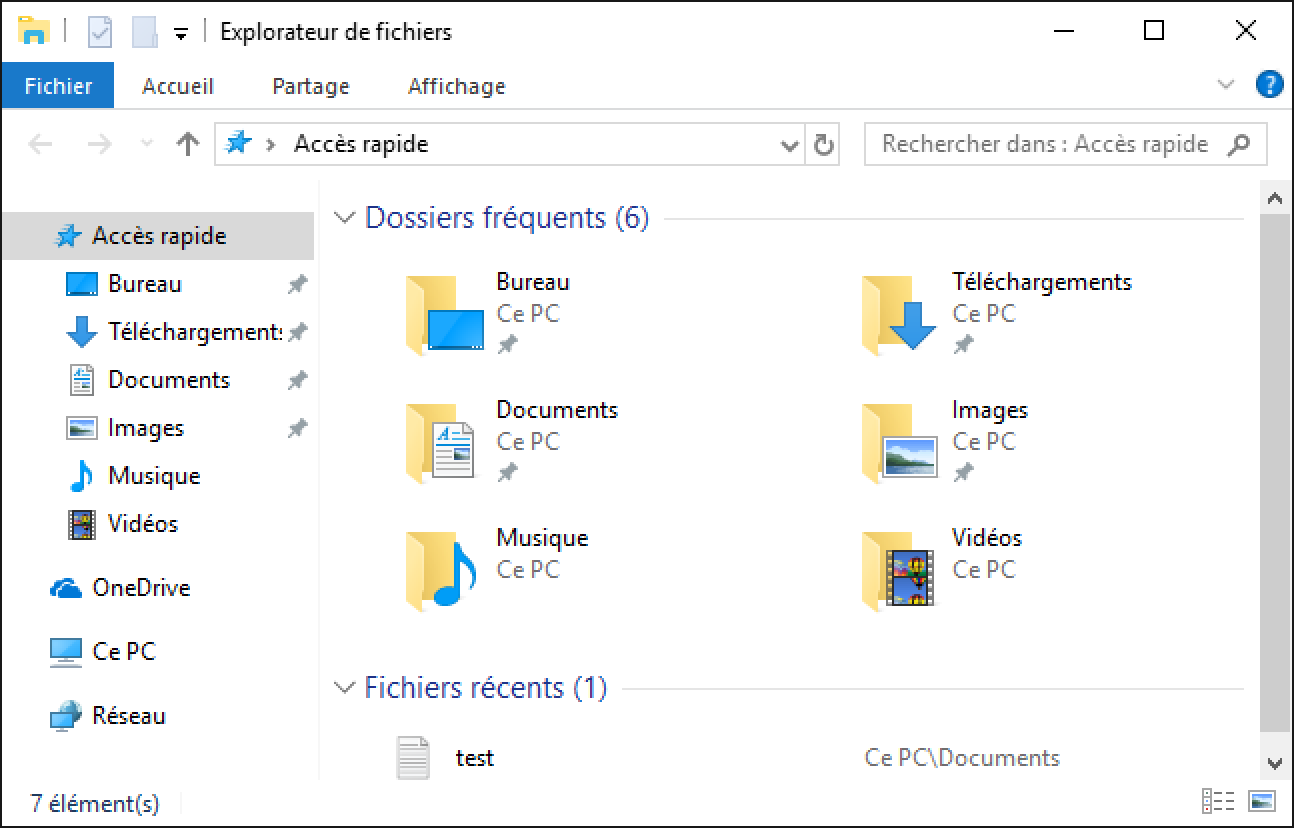
\includegraphics[width=\linewidth]{images/explorer}
  \end{minipage}
  \hfill
  \begin{minipage}{0.48\linewidth}
    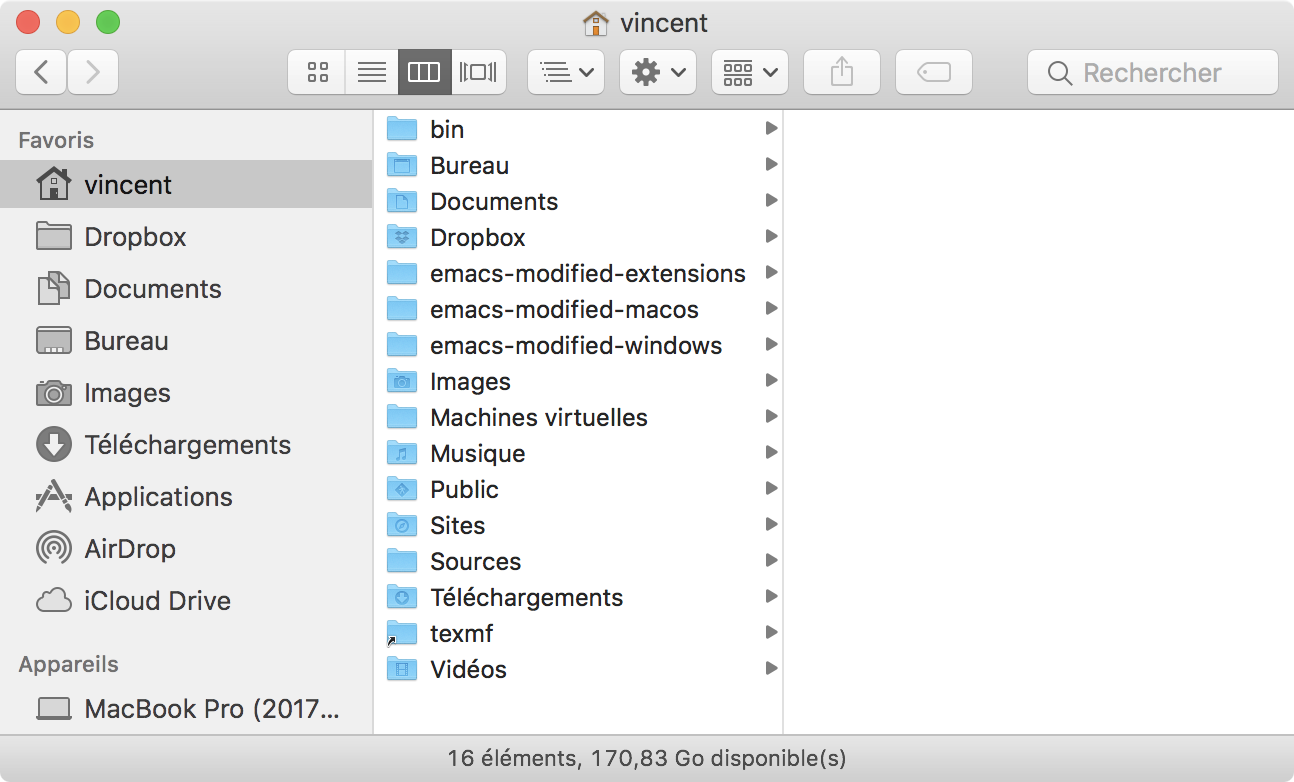
\includegraphics[width=\linewidth]{images/finder}
  \end{minipage}
  \caption[Interfaces graphiques de navigation dans le système de
  fichiers]{Interfaces graphiques de navigation dans le système de
    fichiers: Explorateur Windows (à gauche) et Finder (à droite)}
  \label{fig:informatique:explorer+finder}
\end{figure}

\tipbox{Pour accéder à la racine du système de fichiers dans
  l'Explorateur Windows, il faut ouvrir l'arborescence sous «Ce PC» ou
  «Ordinateur». Dans le Finder de macOS, on atteint la racine en
  sélectionnant «Macintosh~HD» dans la barre latérale.}

\subsection{Particularités du système de fichiers de Windows}
\label{sec:informatique:fs:windows}

Dans Windows, chaque lecteur physique ou lecteur réseau dispose de son
propre arbre de fichiers. La racine est identifiée par une lettre. Le
premier disque dur est \code{C}\footnote{%
  La nomenclature des lecteurs date d'une époque où les ordinateurs
  personnels n'étaient pas tous équipés d'un disque dur, mais plutôt
  d'un ou deux lecteurs de disquettes. Ceux-ci étaient identifiés par
  les lettres \code{A} et \code{B}.}. %
Si le système comporte plus d'un disque, l'utilisateur doit savoir sur
quel disque retrouver ou enregistrer ses données.

Depuis au moins la version~7 de Windows, le répertoire (ou dossier)
personnel des utilisateurs se retrouve sous
\code{C:{\bs}Users}\footnote{%
  Ce répertoire est affiché sous le nom \code{Utilisateurs} dans la
  version française du système d'exploitation.}, %
tel qu'illustré à la \autoref{fig:informatique:fs}. Ainsi, la
véritable position du dossier \code{Documents} d'Alexandre dans le
système de fichiers est \code{C:{\bs}Users{\bs}Alexandre{\bs}Documents}.

\windowsbox{Le répertoire personnel n'est pas affiché par défaut
  dans l'Explorateur Windows. Pour y accéder, vous devez naviguer à
  partir de la racine du système de fichiers dans «Ce PC» ou
  «Ordinateur».}

Le système de fichiers de Windows est insensible à la casse,
c'est-à-dire qu'il ne fait aucune distinction entre \code{Program
  Files}, \code{program files} et \code{PROGRAM FILES}. Dans les
chemins d'accès (voir ci-dessous), la barre oblique inversée
«{\bs}» sépare les noms de répertoires.

\subsection{Particularités du système de fichiers de Unix}
\label{sec:informatique:fs:unix}

La racine du système de fichiers est toujours identifiée par le
symbole «\code{/}» sous \index{Unix}Unix. Les disques, physiques ou
réseau, sont accessibles par divers \emph{points de montage} dans le
système de fichiers.

Pour illustrer, supposons qu'un ordinateur dispose de deux disques
durs; le premier est réservé au système d'exploitation et aux
applications partagées, alors que le second renferme les fichiers
personnels des utilisateurs. Dans un tel scénario, le premier disque
sera monté sur le répertoire \code{/} et le second, sur le répertoire
\code{/home}. Le système de fichier dirigera automatiquement les
requêtes vers le bon disque. L'utilisateur n'a jamais à se préoccuper
de l'organisation physique des disques.

\osxbox{Sous macOS, les clés USB, disques durs externes ou disques
  réseau sont montés dans le répertoire \code{/Volumes}. Le répertoire
  n'existe pas lorsqu'aucun disque externe n'est connecté.}

Tel que mentionné à la section précédente, dans les système Unix le
répertoire personnel des utilisateurs se trouve sous
\code{/Users} (macOS) ou \code{/home} (Linux).

Le système de fichiers sous Unix est généralement sensible à la casse.
La barre oblique «\code{/}» sépare les noms de répertoires dans les
chemins d'accès.

Les fichiers dont le nom débute par un point «\verb=.=» sont des
fichiers cachés. À moins de demander explicitement de les afficher,
ils n'apparaissent donc pas dans la liste des fichiers à la ligne de
commande ou dans les interfaces graphiques.

\subsection{Chemin d'accès}
\label{sec:informatique:fs:path}

Le \index{chemin d'accès}chemin d'accès (\emph{path}) d'un fichier ou
d'un répertoire décrit la position de la ressource dans le système de
fichiers. Un chemin d'accès peut être absolu ou relatif.
\begin{description}
\item[Chemin absolu] \index{chemin d'accès!absolu} La position d'un
  fichier est décrite à partir de la racine, de telle sorte que le
  chemin d'accès demeure valide depuis n'importe quel point dans le
  système de fichier.

  Dans l'extrait de système de fichier Windows de la
  \autoref{fig:informatique:fs}, le chemin d'accès absolu vers le
  fichier \code{synthese-1.doc} est:
\begin{Schunk}
\begin{Verbatim}
C:\Users\Alexandre\Documents\synthese-1.doc
\end{Verbatim}
\end{Schunk}
\item[Chemin relatif] \index{chemin d'accès!relatif} La position d'un
  fichier est donnée à partir d'un endroit précis dans le système de
  fichier autre que la racine. Le chemin dépend donc du répertoire
  courant. On a recours au nom fictif «\verb=..=» pour identifier le
  répertoire parent (un niveau supérieur dans l'arbre des fichiers).

  Par exemple, à partir du répertoire \code{Documents/Cours} de
  Marianne dans le système de fichier Unix de la
  \autoref{fig:informatique:fs}, le chemin d'accès relatif vers le
  fichier \code{freestyle.txt} est:
\begin{Schunk}
\begin{Verbatim}
../../Desktop/freestyle.txt
\end{Verbatim}
\end{Schunk}
\end{description}

La notion de chemin d'accès fait également référence à la liste des
répertoires dans lesquels le système d'exploitation recherche une
application lorsqu'elle est appelée. Cette liste est conservée dans
une variable d'environnement nommée \verb=%PATH%= sous Windows
et \verb=$PATH= sous \index{Unix}Unix. Il est hors de la portée de ce
document d'expliquer comment modifier la variable d'environnement. La
réponse se trouve à une requête près dans un moteur de recherche.


\section{Exercices}
\label{operateurs:exercices}

\Opensolutionfile{solutions}[solutions-informatique]

\begin{Filesave}{solutions}
\section*{Chapitre \ref*{chap:informatique}}
\addcontentsline{toc}{section}{Chapitre \protect\ref*{chap:informatique}}

\end{Filesave}

\begin{exercice}[nosol]
  Des nouveaux langages de programmation apparaissent régulièrement.
  Deux exemples récents provenant de géants de l'industrie sont
  \link{https://swift.org}{Swift}, de Apple, et
  \link{https://golang.org}{Go}, de Google. À partir des informations
  glanées sur les sites Internet des langages et dans les pages
  Wikipedia qui leurs sont consacrées, retracer les grands langages
  ayant servi comme sources d'inspiration à \index{Swift}Swift et à
  \index{Go}Go.
\end{exercice}

\begin{exercice}
  Soit $A$, $B$, $C$ et $D$ quatre nombres. L'opération en notation
  infixée
  \begin{equation*}
    A \times B + C \div D
  \end{equation*}
  s'écrit
  \begin{equation*}
    +\, \times\, A\; B\, \div\, C\; D
  \end{equation*}
  en notation préfixée et
  \begin{equation*}
    A\; B\, \times\, C\; D\, \div +
  \end{equation*}
  en notation suffixée.
  \begin{enumerate}
  \item Exprimer en notations préfixée et suffixée l'opération en
    notation infixée suivante:
    \begin{equation*}
      A \times (B + C) \div D.
    \end{equation*}
  \item Les opérations suivantes exprimées en notation préfixée et
    suffixée, dans l'ordre, effectuent la même opération arithmétique.
    \begin{gather*}
      \times\, A\, +\, B\, \div\, C\; D \\
      A\; B\; C\; D\, \div +\, \times
    \end{gather*}
    Exprimer cette opération en notation infixée.
  \end{enumerate}
  \begin{sol}
    \begin{enumerate}
    \item $\div \times\, A\, +\, B\; C\; D$ en notation préfixée;
      $A\; B\; C\, +\, \times\, D\, \div$ en notation suffixée.
    \item $A \times (B + C \div D)$
    \end{enumerate}
  \end{sol}
\end{exercice}

\begin{exercice}[nosol]
  Les répertoires \code{Documents} et \code{Desktop} (ou \code{Bureau}
  dans la version française) existent par défaut dans le
  \index{repertoire personnel@répertoire personnel}répertoire
  personnel des utilisateurs tant dans macOS que dans Windows.
  Localiser ces deux répertoires dans le système de fichier à partir
  de la racine avec l'Explorateur Windows ou le Finder.
\end{exercice}

\Closesolutionfile{solutions}

%%% Local Variables:
%%% mode: latex
%%% TeX-engine: xetex
%%% TeX-master: "programmer-avec-r"
%%% coding: utf-8
%%% End:
